\section{Ejercicio 4}

\subsection{Introducción}
\paragraph{}
En este ejercicio, nos fue requerida una implementación de un algoritmo que utilice la técnica de búsqueda local para resolver el problema de \mc.

\subsection{Explicación}

\paragraph{}
La idea general de la búsqueda local es partir de una solución parcial, ya sea una dada por algún algoritmo constructivo o alguna solución trivial y de allí realizar una búsqueda de soluciones vecinas que pueda mejorar la solución parcial encontrada antes.

\paragraph{}
Para comenzar con el algoritmo, se decidió que la solución de partida sea la que se obtiene a partir del algoritmo constructivo implementado como solución del ejercicio 3, que se detalla en la sección [\ref{ej3}].\\
Luego, se definió qué iba a ser tomado como vecindad, es decir, qué conjunto de soluciones iban a ser tenidas en cuenta a la hora de realizar la búsqueda local. Para definir esta vecindad, hubo que tener en cuenta que la misma debía ser fácil de calcular. Además, el criterio de parada debía ser cuando se encontrara un máximo local.

\paragraph{}
Como la vecindad a definir debía ser lo suficientemente simple y debía mantener un espacio de búsqueda de soluciones relativamente pequeño, se optó por definir la siguiente vecindad:\\
Dada una solución parcial $S$, se saca un nodo $v$ de dicha solución y se obtiene $S_1 = S\ \diagdown\ \{v\}$, y se define un conjunto de candidatos a mejorar la solución parcial $S$. Sea $C$ este conjunto de candidatos, los vértices pertenecientes a $C$ son todos aquellos pertenecientes al grafo original que tienen al menos un vecino dentro de $S_1$. Una vez obtenido el conjunto de candidatos, se los va tomando en orden de grados (de mayor a menor) y se intenta insertarlos en $S_1$ siempre que esa inserción mantenga la propiedad de que $S_1$ sea una clique. Una vez hecho el intento con todos los vértices de $C$ se verifica si se obtuvo o no una mejor solución que $S$, es decir, si $\#S_1\ > \#S$. De ser positivo, esta solución $S_1$ es guardada.\\
Estos pasos se repiten para todos los vértices pertenecientes a $S$. Una vez finalizado esto, pueden suceder 2 cosas: que se haya encontrado una mejor solución que $S$ o que no. Si se encontró una mejor solución, entonces se repiten todos los pasos antes mencionados pero para esta nueva solución parcial. Sino, significa que se encontró un máximo local, por lo que el algoritmo finaliza. Así como el orden en que se van tomando los vértices de $C$ es de mayor a menor grado, en el caso de los vértices que se van descartando de $S$ se hace en orden inverso, es decir, comenzando por los que tienen menor grado hacia los que tienen mayor grado.

\paragraph{}
Para graficar mejor este procedimiento, se detalla a continuación el pseudocódigo de las funciones que lo implementan. Recordar que dentro de los comentarios que contienen la complejidad, la letra ``n'' representa la cantidad de nodos de un grafo.

\vspace{2em}
\incmargin{1em}
\linesnumbered
\restylealgo{boxed}
\footnotesize 
\textbf{busquedaLocal}(G: grafo) \\
\begin{algorithm}[H]
	\BlankLine
	termine = false\tcp*{\Ode{1}}

	maxClique = cliqueConstructivo(G)\tcp*{\Ode{n^3}}
	
	\textbf{mientras} termine $==$ false \textbf{hacer}\\
		
		\tab cambio = false\tcp*{\Ode{1}}

		\tab $<$maxClique,cambio$> =$ cambiarSiMaximiza(G,maxClique,cambio)\tcp*{\Ode{n^3 * log(n)}}
		
		\tab \textbf{si} cambio $==$ false\tcp*{\Ode{1}}
			\tab \tab termine = true\tcp*{\Ode{1}}
		\tab \textbf{fin si}\\
	\textbf{fin mientras}\\

	\textbf{devolver} maxClique

\caption{Pseudocódigo del algoritmo de búsqueda local}
\end{algorithm}

\vspace{3em}


\textbf{cambiarSiMaximiza}(G: grafo, maxClique: conjunto, cambio: bool) \\
\begin{algorithm}[H]
	\BlankLine
	copiaClique = maxClique\tcp*{\Ode{n}}
	cliqueDeMenorAMayor = deCliqueAMinHeap(copiaClique)\tcp*{\Ode{n*log(n)}}

	\textbf{mientras} cliqueDeMenorAMayor \textbf{no sea un Heap vacío}\\

		\tab posibleMejora = copiaClique $\diagdown$ \{tope(cliqueDeMenorAMayor)\}\tcp*{\Ode{log(n)}}

		\tab candidatos = vecinosAMaxHeap(posibleMejora)\tcp*{\Ode{n^2 * log(n)}}
		
		\tab \textbf{mientras} candidatos \textbf{no sea un Heap vacío}\\
			\tab \tab \textbf{si} vecinoDeTodos(tope(candidatos),posibleMejora)\tcp*{\Ode{n}}
				\tab \tab \tab posibleMejora = posibleMejora $\cup$ tope(candidatos)\tcp*{\Ode{log(n)}}
			\tab \tab \textbf{fin si}\\
			\tab \tab pop(candidatos)\tcp*{\Ode{log(n)}}
		\tab \textbf{fin mientras}\\


		\tab \textbf{si} $\#$posibleMejora $>\ \#$maxClique\\
			\tab \tab maxClique = posibleMejora\tcp*{\Ode{n}}
			\tab \tab cambio = true\tcp*{\Ode{1}}
		\tab \textbf{fin si}\\
		\tab pop(cliqueDeMenorAMayor)\tcp*{\Ode{log(n)}}
	\textbf{fin mientras}\\

	\textbf{devolver} $<$maxClique,cambio$>$

\caption{Pseudocódigo del algoritmo cambiarSiMaximiza}
\end{algorithm}

\vspace{3em}



\normalsize
\subsection{Análisis de la complejidad del algoritmo}
\label{complejidad4}
\paragraph{}
Para analizar la complejidad del algoritmo de búsqueda local basta con comprender cómo se comporta tanto el algoritmo principal, llamado ``busquedaLocal'', como el secundario llamado ``cambiarSiMaximiza''. El resto de los algoritmos puede obviarse ya que, o bien ya fueron analizados en la sección [\ref{ej3}] como es el caso de ``vecinoDeTodos'', o bien tienen un comportamiento trivial y conocido, como es el caso de las funciones ``deCliqueAMinHeap'' y ``vecinosAMaxHeap'' que como sus nombres lo indican, son funciones que devuelven un min-heap y un max-heap respectivamente. Lo que si es interesante aclarar de estas funciones es qué elementos devuelven en cada heap. En el caso de ``deCliqueAMinHeap'' toma todos los vértices que pertenecen a la clique que se le pasa como parámetro y los heapifica según sus grados (de menor a mayor). En cambio, la función ``vecinosAMaxHeap'' toma todos aquellos vértices que no pertenecen a la clique pero que tienen algún vecino dentro de ella y los inserta en un max-heap ordenándolos por grado.

\paragraph{}
En primer lugar vamos a analizar al segundo algoritmo aquí presentado, es decir, ``cambiarSiMaximiza''. Como se observa dentro del pseudocódigo, existen dos ciclos dentro del algoritmo, uno dentro de otro. Para que el ciclo más global finalice, debe ejecutarse tantas veces como elementos haya en ``cliqueDeMenorAMayor'' por lo que a lo sumo se ejecutará $n$ veces. Pasa lo mismo con el ciclo anidado dentro de este. El mismo se ejecutará tantas veces como vecinos de la clique haya, es decir, a lo sumo $n$. Dentro de este segundo ciclo, la función más costosa es la que se encuentra en la guarda del $if$ que tiene una complejidad de \Ode{n}. Como este ciclo se ejecuta a lo sumo $n$ veces, la complejidad del mismo es \Ode{n^2}. Ahora bien, además del ciclo anidado, la otra función costosa dentro del ciclo mayor es ``vecinosAMaxHeap'' que cuesta \Ode{n^2 * log(n)}. Por lo tanto, como el ciclo mayor se ejecuta a lo sumo $n$ veces, la complejidad total de este algoritmo es \Ode{n^3 * log(n)}.

\paragraph{}
Ahora bien, sólo faltaría analizar qué complejidad tiene la función principal. Pero si se observa bien, este algoritmo consta de un ciclo en el cuál existe una llamada a la función antes analizada. Por lo cuál sabiendo cuántas veces se ejecuta este ciclo, sabremos la complejidad total del algoritmo. Este ciclo finaliza cuando la variable ``termine'' valga $true$. La misma tomará este valor, cuando la variable ``cambio'' valga $false$ luego del llamado a ``cambiarSiMaximiza''. Por lo tanto, hay que volver al pseudocódigo de esta función para saber cómo se comporta allí esta variable.

\paragraph{}
La variable ``cambio'' sólo se modifica cuando existe una mejora en la clique mayor temporalmente hallada. Podemos ver entonces que el peor caso se da cuando la clique mayor temporal comienza con tamaño igual a 1 (respuesta obtenida con el algoritmo constructivo). Luego, dentro de cada llamada a la función ``cambiarSiMaximiza'', lo peor sería que sólo exista una mejora del tamaño en una unidad, es decir, en el primer llamado habrá un cambio de tamaño de 1 a 2, por lo que la variable ``cambio'' tomará el valor de verdad $true$. Cómo cada vez que se llama a esta función, esta mejora la respuesta temporal en una unidad, se puede observar que en el n-ésimo llamado el tamaño de la clique mayor temporal no aumentará, ya que se introdujeron todos los vértices existentes, por lo que en este llamado a la función secundaria, el algoritmo no entrará al $if$ en el que se modifica a la variable ``cambio'', por lo que dicha variable quedará con valor $false$\footnote{cabe notar que en cada llamado a la función ``cambiarSiMaximiza'' esta variable entra con valor $false$}. Por lo tanto, en el peor caso, en el n-ésimo llamado a esta función, la guarda del ciclo de la función principal se hace falsa. Entonces, como dicho ciclo se ejecutará a lo sumo $n$ veces, y en el mismo hay un llamado a una función de complejidad \Ode{n^3 * log(n)}, la complejidad total del algoritmo principal es \Ode{n^4 * log(n)}.



\subsection{Resultados}
\paragraph{}
A continuación se presentan los gráficos provenientes de las pruebas realizadas con archivos generados al azar. La forma en la que fueron generados estos archivos de entrada es explicada en la sección [\ref{anexo}].

%primeras 2 imagenes
\begin{figure}[htb]
    \begin{minipage}{\textwidth}
	\begin{center}
		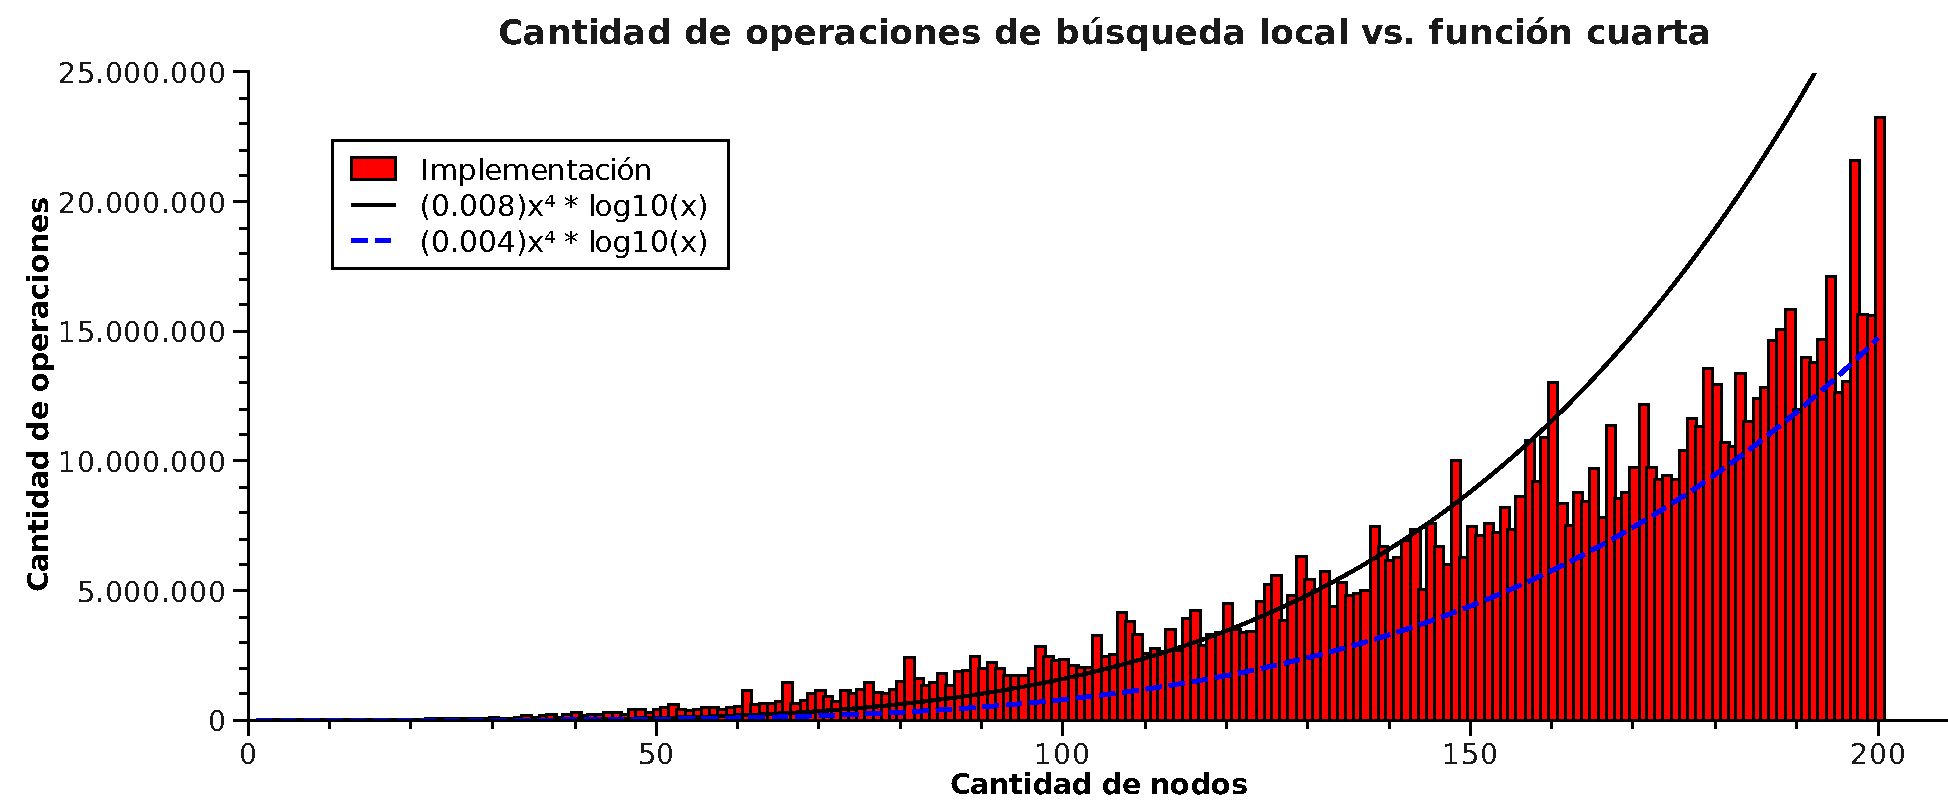
\includegraphics[width=\textwidth]{./otros/graficos/operaciones_200nodos1_ej4.pdf}
		\caption{Muestra el comportamiento del algoritmo de búsqueda local, comparando cantidad de nodos contra cantidad de operaciones. La probabilidad de aparición de ejes en esta muestra fue del 50\%}
		\label{ej4contarOp}
	\end{center}
    \end{minipage}

\vspace*{1cm}

    \begin{minipage}{\textwidth}
	\begin{center}
		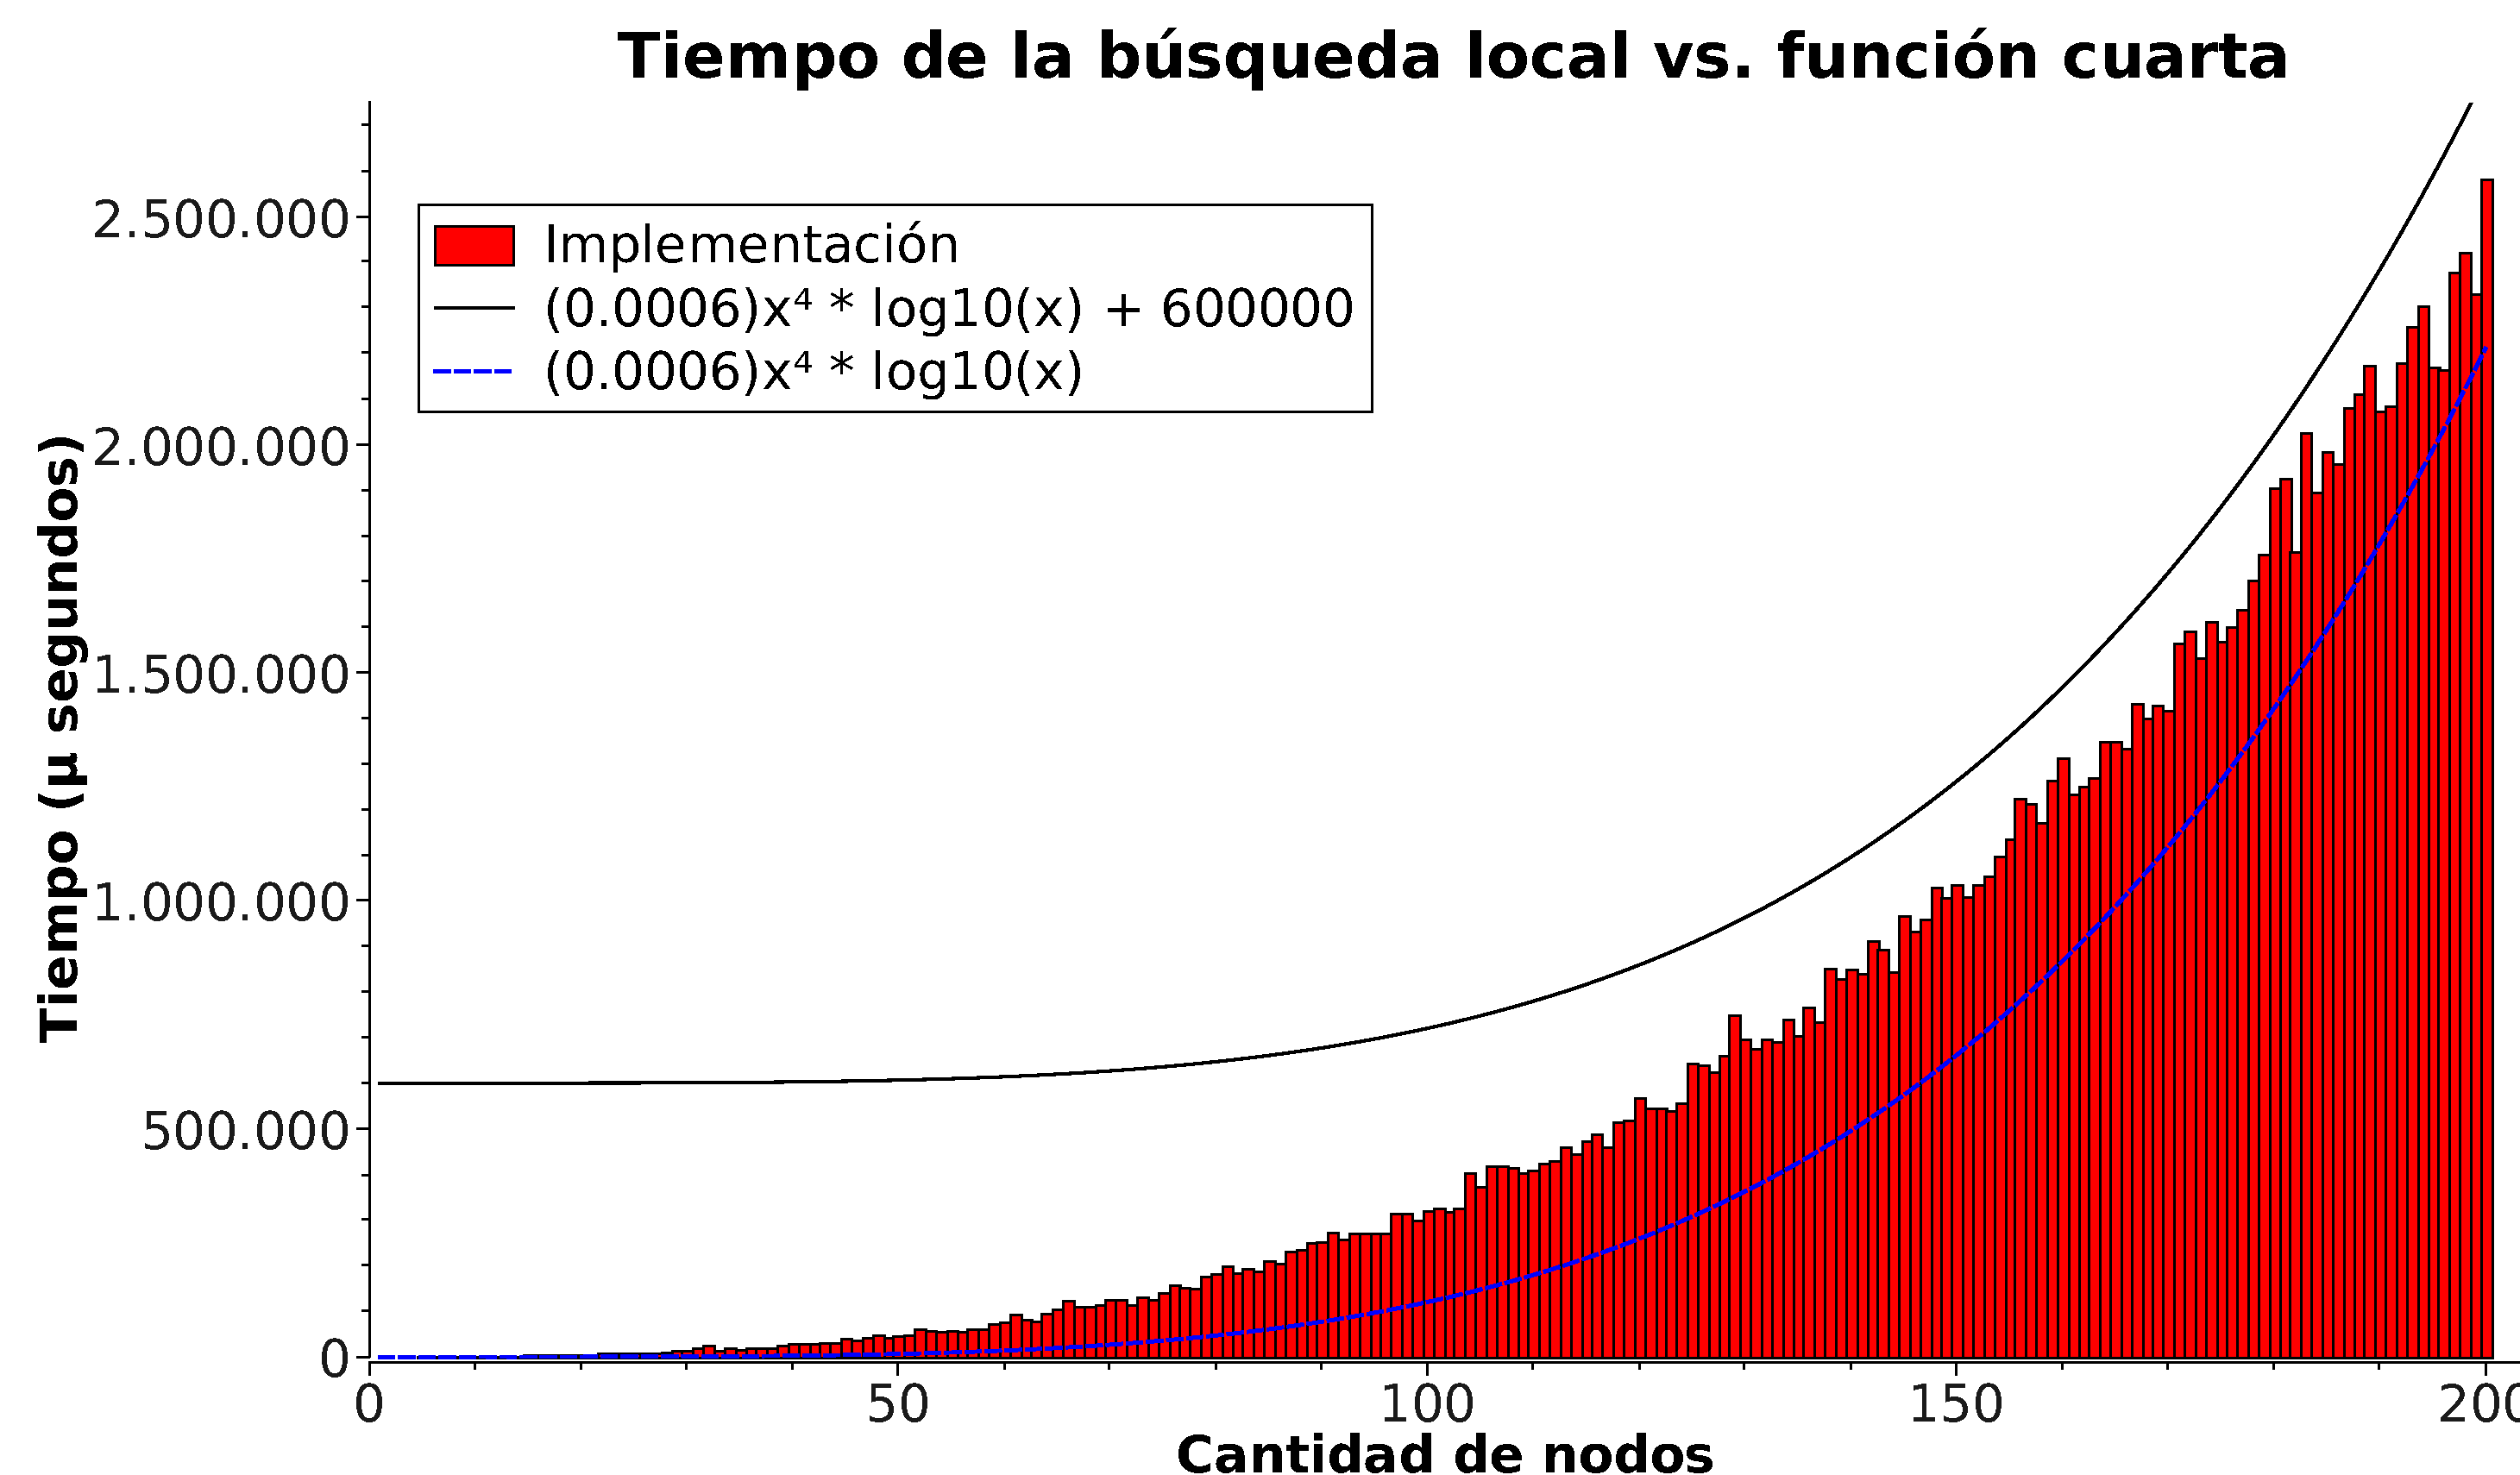
\includegraphics[width=\textwidth]{./otros/graficos/tiempo_200nodos1_ej4.pdf}
		\caption{Muestra el comportamiento del algoritmo de búsqueda local, comparando cantidad de nodos contra el tiempo medido en microsegundos. La probabilidad de aparición de ejes en esta muestra fue del 50\%}
		\label{ej4contarTiempo}
	\end{center}
    \end{minipage}

\end{figure}

\subsection{Debate y conclusiones}
\paragraph{}
Según los datos arrojados por los gráficos en la sección anterior, podemos ver que los datos arrojados por las distintas corridas del algoritmo de búsqueda local tienen la forma que se esperaba. En la sección [\ref{complejidad4}], se explicó y analizó la complejidad de esta heurística, y se concluyó que la misma era \Ode{n^4 * log(n)}. Dentro de estos gráficos, se ve que en estos casos de prueba, la heurística parece haberse comportado como era esperado, y pudo ser acotada por arriba y abajo por una función cuarta multiplicada por un logaritmo.

\paragraph{}
Como se comentó en la sección de debate y conclusiones del ejercicio 3, a pesar de haberse tomado varias muestras en las que se variaba el número de ejes y de nodos, todos los resultados presentaban la misma forma, salvo alguna constante no muy pronunciada. Por ello no pareció adecuado incluir más gráficos, ya que en general y utilizando los generadores implementados por el grupo para este trabajo práctico, el comportamiento no varió de muestra en muestra.

\paragraph{}
Podemos concluir entonces que el algoritmo, tanto en la teoría como en la práctica para los casos de prueba realizados se comportó como se esperaba, arrojando una complejidad de \Ode{n^4 * log(n)}.

